% % % % % % % % % % % % % % % % % % % % % % % % % % % % % % % % % % % % 
% 
% FS-Vorlage											Stand: 30.01.12
%
% Formelsammlungsvorlage von Emanuel Regnath und Martin Zellner	
% Bietet verschiedene Abkürzungen und Befehle	
%
% % % % % % % % % % % % % % % % % % % % % % % % % % % % % % % % % % % % 


% Dokumenteinstellungen
% ======================================================================

% Dokumentklasse
\documentclass[german]{latex4ei/latex4ei_sheet}


\usepackage{amsmath, amssymb, amsfonts}  % For mathematical symbols and environments
\usepackage{mathtools}                   % Enhancements for amsmath
\usepackage{tabularx}                    % For tables with flexible width
\usepackage{graphicx}                    % For including graphics and scaling
\usepackage{tikz}                        % For drawing vector graphics
\usepackage{physics}                     % For derivatives, integrals, and bra-ket notation
\usepackage{xcolor}                      % Color options for annotations
\usepackage{cancel}                      % For canceling terms
\usepackage{bm}                          % Bold math for vectors
\usepackage{empheq}                      % Emphasized equations
\usepackage{trsym,trfsigns}

% Befehle Signaldarstellung:
\newcommand{\Trans}[1]{\TransSymb\left\{#1\right\}}	% LTI-Transformation

\renewcommand{\diff}{\mathop{}\!\mathrm{\vphantom( d}}

\renewcommand{\laplace}{\Laplace}

\title{Signaltheorie}

% Dokumentbeginn
% ======================================================================
\begin{document}


% ---------------------------------------
% | 		Signaldarstellung			|
% ~~~~~~~~~~~~~~~~~~~~~~~~~~~~~~~~~~~~~~~
%=======================================================================
\maketitle
	%Erst skalieren um $\frac{1}{a}$, dann verschieben um $b$! Form: $a(t-b)$\\#
	%\emph{Hinweis:} Im Modul Signaldarstellung ist keine Formelsammlung im üblichen Sinn zugelassen. Deshalb ist dies nur eine Sammlung von Informationen, die auf den freien Seiten im Manuskript Platz finden können.

	\section{Additionstheoreme}
	\begin{sectionbox}
		\subsection{sinh, cosh \quad $\cosh^2(x)  - \sinh^2(x) = 1$}
			$\sinh x = \frac{1}{2}(e^x -e^{-x}) \qquad \quad \operatorname{arsinh}\ x:= \ln\left(x+\sqrt{x^2+1}\right) \\
			\cosh x  = \frac{1}{2}(e^x +e^{-x}) \qquad \quad \operatorname{arcosh}\ x:= \ln\left(x+\sqrt{x^2-1}\right)$

			\begin{tabular}{ll}
				Additionstheoreme &	Stammfunktionen \\
				$\cosh x \,\; + \sinh x \,\,= e^{x}$ & $\int \sinh x \, dx = \cosh x + C$\\
				$\sinh({\rm arcosh}(x)) = \sqrt{x^2 - 1}$ & $\int \cosh x \, dx = \sinh x + C $\\
				$\cosh({\rm arsinh}(x)) = \sqrt{x^2 + 1}$ 	
			\end{tabular}
		\subsection{sin, cos \quad $\sin^2(x)  + \cos^2(x) = 1$}
			$\begin{array}{c|c|c|c|c|c|c|c|c}
				x & 0 & \pi / 6 & \pi / 4 & \pi / 3 & \pi / 2 & \pi & \frac{3}{2}\pi & 2 \pi \\ \hline
				\sin & 0 & \frac{1}{2} & \frac{1}{\sqrt{2}} & \frac{\sqrt 3}{2} & 1 & 0 & -1 & 0 \\
				\cos & 1 & \frac{\sqrt 3}{2} & \frac{1}{\sqrt 2} & \frac{1}{2} & 0 & -1 & 0 & 1 \\     
				\tan & 0 & \frac{\sqrt{3}}{3}&	1				 &	\sqrt{3} & \infty & 0 & - \infty & 0\\
			\end{array}$ 
			\begin{tabular}{l  l} 
				Additionstheoreme &  Stammfunktionen\\
		 		$\cos (x - \frac{\pi}{2}) = \sin x$ & $\int x \cos(x) \diff x = \cos(x) + x \sin(x)$\\
				$\sin (x + \frac{\pi}{2}) = \cos x$ & $\int x \sin(x) \diff x = \sin(x) - x \cos(x)$\\
			 	$\sin 2x = 2 \sin x \cos x $  & $\int \sin^2(x) \diff x = \frac12 \bigl(x - \sin(x)\cos(x) \bigr)$\\
			 	$\cos 2x = 2\cos^2 x - 1$  & $\int \cos^2(x) \diff x = \frac12 \bigl(x + \sin(x)\cos(x) \bigr)$\\
		 		$\sin(x) = \tan(x)\cos(x)$ & $\int \cos(x)\sin(x) = -\frac12 \cos^2(x)$ \\
			\end{tabular}

			$\sin x = \frac{1}{2\i} ( e^{\i x} - e^{- \i x})$ \qquad $\cos x = \frac{1}{2}( e^{\i x} + e^{- \i x})$
	\end{sectionbox}
	\section{Signaldarstellung}
	\begin{sectionbox}
	% Login: sd convolution
	\subsection{Signale \& Systeme}
	Allgemeine Form: $x_i(t) = \underbrace{g}_{\textcircled{3}} \cdot [x(\underbrace{s}_{\textcircled{2}} \cdot t + \underbrace{v}_{\textcircled{1}})] + \underbrace{r}_{\textcircled{4}}$
	\begin{itemize}
		\item \textcircled{1}: Translation $\rightleftarrows$
		\item \textcircled{2}: Skalierung $\longleftrightarrow$
		\item \textcircled{3}: Gewichtung $\updownarrow$
		\item \textcircled{4}: Verschiebung $\downarrow\uparrow$
	\end{itemize}
%	$x(t) \rightarrow x(t - 1)$ Verschiebung um $1$ in $x$-Richtung \\
%	$x(t) \rightarrow x(2 t)$ Stauchung um $2$ in $x$-Richtung \\
%	$x(t) \rightarrow x(-t)$ Spiegelung an der $y$-Achse
%	Linearität (L): $a x_1(t) + b x_2(t) \rightarrow a y_1(t) + b y_2(t)$ \\
%	Zeitinvarianz (TI): $x(t - t_0) \rightarrow y (t-t_0)$
	\end{sectionbox}
	\subsection{Analytische Darstellung, Stochastische Darstellung}
	\begin{sectionbox}
	Zeitkontinuierliches Signal $x(t)$ und diskretes Signal $x[n]$\\
	
%	\emph{Abtastung}\\
%	$\rightarrow$ S. 10
%	$x(t) \stackrel{\text{jede} T_S}{\rightarrow} x[t] \stackrel{\text{mit} n = \frac{t}{T_S}}{\rightarrow} x[n]$\\
%	$\Rightarrow x[n] = \sum\limits_{n = -\Delta}^\Delta x(t) \cdot \delta[t - n T_s]$\\
%	$T_S$: Abtastweite
	\subsubsection{Besondere Grundfunktionen}
	\emph{Einheitsimpuls} $\delta[n - n_0] = \begin{cases}
		1, & n = n_0\\
		0, & n \neq n_0\\
	\end{cases}$\\
	\emph{Zeitdiskreter Einheitssprung} $u[n - n_0] = \begin{cases}
		1, & n \geq n_0\\
		0, & n < n_0\\
	\end{cases}$\\
	oder $u[n] = \sum\limits_{l=0}^{\infty}{\delta[n - l]}$\\
	\emph{Diracsche $\delta$-Funktion}\\
	$\int\limits_{-\infty}^{\infty}{\delta(t - t_0)} = 1$ und $\delta(t - t_0) = \begin{cases} %
		\infty, & t = t_0\\
		0, & t \neq t_0\\
	\end{cases}$\\
	$\int\limits_{-\infty}^{\infty}{f(t)\delta(t - t_0)\diff t} = f(t_0)$\\
	$\int\limits_{-\infty}^{\infty}{e^{\pm j \omega t}\delta(t) \diff t} = 1$ und $\delta(t) = \frac{1}{2 \pi}\int\limits_{-\infty}^{\infty}{e^{\pm j \omega t}\diff \omega}$\\
	\emph{Zeitkontinuierlicher Einheitssprung} $u(t - t_0) = \begin{cases}
		1, & t \geq t_0\\
		0, & t < t_0\\
	\end{cases}$\\
	Es gilt: $u(t - t_0) = \int\limits_{-\infty}^{t}{\delta(\tau - t_0)\diff\tau}$
%	
%	Einheitsimpuls $\delta[n-n_0] = \delta_{n,n_0}$\\
%	Abtastweite $T_S$\\
%	Abtastung $X[t] = i(t) \cdot X(t) = \sum\limits_{n = -\Delta}^\Delta x(t) \cdot \delta[t-n T_s]$\\
%	
%	
%	Sprungfunktion: $\delta_\varepsilon(t-t_0)$\\
%	Einheizsprung: $\heavi(t-t_0)$\\
	\end{sectionbox}
	\subsection{LTI-Systeme}
	\begin{sectionbox}
	Alle Angaben gelten gleichermaßen für zeitdiskrete Signale.\\
	i. Allg. lin. DGL: $a_0 y + a_1 \dot{y} + a_2 \ddot{y} + \dots = b_0 x + b_1 \dot{x} + b_2 \ddot{x} + \dots$
	\boxed{y(t) = T\{x(t)\}}
	\begin{tabular}{@{}lll}
		& Input & Output\\
		\emph{linear} & $a x_1(t) + b x_2(t)$ & $\Rightarrow a y_1(t) + b y_2(t)$\\
		\emph{zeitinvariant} & $x(t-t_0)$ & $\Rightarrow y(t-t_0)$\\
	\end{tabular}
	
	Sprungantwort $s(t)$ auf $x(t) = u(t)$\\
	Impulsantwort $h(t) = \dot s(t)$ auf $x(t) = \delta(t)$
	
	Lösungsmöglichkeiten:\\
	1. Lösen der DGL \qquad 2. Faltungsintegral\\
	
	\subsubsection*{Faltung mit Folie}
	Gebrauchte Hilfsmittel: Klarsichtfolie, Folienstift\\
	$x(t) \ast h(t) = \int\limits_{-\infty}^{\infty}{\underbrace{x(\tau)}_{\textcircled{1}} \underbrace{h(t - \tau)}_{\textcircled{2}} \diff \tau}$
	\begin{enumerate}
		\item \textcircled{2} auf Folie übertragen
		\item $t$ im Ursprung
		\item Folie nach links drehen
		\item Beschriften: $h(t - \tau) \begin{cases}
			\text{rechts von }t: t + \cdots\\
			\text{links von }t: t - \cdots\\
		\end{cases}$
		\item Folie über \textcircled{1} schieben
		\item Keine Überlappung $\Rightarrow y = 0$
		\item Integration in stetige Bereiche aufteilen
		\item Grenzen bestimmen
		\item \textcircled{1} abschnittsweise analytisch beschreiben
		\item \textcircled{2} abschnittsweise analytisch beschreiben
		\item Teilintegrale lösen
	\end{enumerate}
	\end{sectionbox}
	\subsection{Faltung von Funktionen}
	\begin{sectionbox}
	\boxed{\begin{tabular}{ll} 
	Kontinuierlich: & $(f*g)(x) = \int\limits_{-\infty}^{\infty} f(\tau) g(t-\tau) \diff \tau$\\[0.5em]
	Diskret: & $(f*g)[n] = \sum\limits_{k = -\infty}^{\infty} {f[k] g[n-k]}$\\
	\end{tabular}}
	
	\emph{Eigenschaften der Faltungsintegrale(-summen)}\\
	Gültigkeit gleichermaßen für \emph{diskrete} Signale\\
	\begin{tabularx}{\linewidth}{m{1.5cm}X}
		Kommutativität & $f(t)*g(t) = g(t)*f(t)$\\
		Assoziativität & $f(t)*(g(t)*h(t)) = (f(t)*g(t))*h(t)$ \newline (Serienschaltung)\\
		Distributivität & $f(t)*(g(t) + h(t)) = f(t)*g(t) + f(t)*h(t)$ \newline (Parallelschaltung)\\
		Faltung mit Dirac & $x(t)*\delta(t-b) = x(t-b)$ \newline (Gleiches Signal verschoben)\\
		Stabilität & $\int_{-\infty}^{\infty}{\abs{h(\tau)} \diff \tau}<\infty$ \newline $\sum_{l=-\infty}^{\infty}{\abs{h[l]}}<\infty$\\
		Kausalität & $h(t - \tau) = 0$ für $\tau > t$ \newline $h[n - l] = 0$ für $l > n$\\
	\end{tabularx}
	
	\subsubsection*{Spezialfall}
	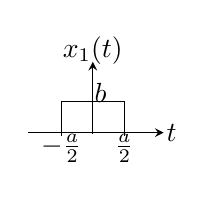
\begin{tikzpicture}[scale=0.2]
		% Gitter zeichnen
		%\draw[help lines] (-4,0) grid (4,4);
		
		% Koordinatenachsen zeichnen
		\begin{scope}[>=stealth]
			\draw[->] (-4.1,0) to (4.5,0);
			\draw[->] (0,-0.1) to (0,4.5);
		\end{scope}
		
		% Achsenbeschriftungen eintragen
		\node (t-Axis) at (5,0) {$t$};
		\node (x-Axis) at (0,5.2) {$x_1(t)$};
		
		% Graph zeichnen
		\draw plot coordinates {(-2,0) (-2,2) (2,2) (2,0)};
		
		% Achsenmarkierungen
		\draw (-2,-0.2) to (-2,0.2);
		\draw (2,-0.2) to (2,0.2);
		\draw (-0.2,2) to (0.2,2);
		\node at (-2,-1) {$-\frac{a}{2}$};
		\node at (2,-1) {$\frac{a}{2}$};
		\node at (0.5,2.5) {$b$};
	\end{tikzpicture}
	\raisebox{0.8cm}{$*$}
	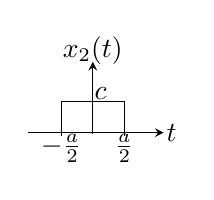
\begin{tikzpicture}[scale=0.2]
			% Gitter zeichnen
			%\draw[help lines] (-4,0) grid (4,4);
			
			% Koordinatenachsen zeichnen
			\begin{scope}[>=stealth]
				\draw[->] (-4.1,0) to (4.5,0);
				\draw[->] (0,-0.1) to (0,4.5);
			\end{scope}
			
			% Achsenbeschriftungen eintragen
			\node (t-Axis) at (5,0) {$t$};
			\node (x-Axis) at (0,5.2) {$x_2(t)$};
			
			% Graph zeichnen
			\draw plot coordinates {(-2,0) (-2,2) (2,2) (2,0)};
			
			% Achsenmarkierungen
			\draw (-2,-0.2) to (-2,0.2);
			\draw (2,-0.2) to (2,0.2);
			\draw (-0.2,2) to (0.2,2);
			\node at (-2,-1) {$-\frac{a}{2}$};
			\node at (2,-1) {$\frac{a}{2}$};
			\node at (0.5,2.5) {$c$};
	\end{tikzpicture}
	\raisebox{0.8cm}{$=$}
	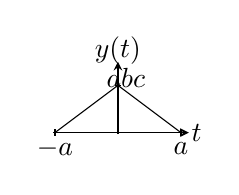
\begin{tikzpicture}[scale=0.2]
			% Gitter zeichnen
			%\draw[help lines] (-4,0) grid (4,4);
			
			% Koordinatenachsen zeichnen
			\begin{scope}[>=stealth]
				\draw[->] (-4.1,0) to (4.5,0);
				\draw[->] (0,-0.1) to (0,4.5);
			\end{scope}
			
			% Achsenbeschriftungen eintragen
			\node (t-Axis) at (5,0) {$t$};
			\node (x-Axis) at (0,5.2) {$y(t)$};
			
			% Graph zeichnen
			\draw plot coordinates {(-4,0) (0,3) (4,0)};
			
			% Achsenmarkierungen
			\draw (-4,-0.2) to (-4,0.2);
			\draw (4,-0.2) to (4,0.2);
			\draw (-0.2,3) to (0.2,3);
			\node at (-4,-1) {$-a$};
			\node at (4,-1) {$a$};
			\node at (0.5,3.5) {$abc$};
	\end{tikzpicture}
%	\\
%	Auf eine Impulsstörung $\delta(t)$ folgt die Impulsantwort $h(t)$\\
%	Jedes Eingangssignal lässt sich als Überlagerung von gewichteten Impulsen darstellen:
%	$x(t) = \int\limits_{-\infty}^{\infty} x(\tau) \delta(t-\tau) \diff \tau$\\
%	Wegen Superposition bei LTI Systemen ist das Ausgangssignal eine Überlagerung von Impulsantworten $y(t) = \int\limits_{-\infty}^{\infty} x(\tau) h(t-\tau) \diff \tau$\\
%	\\
%	Verknüpfung von LTI Systemen:\\
%	Serienschaltung: $y(t) = x(t) * h_1(t) * h_2(t)$\\
%	Prallelschaltung: $y(t) = x(t) * (h_1(t) + h_2(t))$\\
%	% dritte Art?
%	%Faltung von zwei periodischen Signalen:
%	
	
	\subsection{Korrelation (Ähnlichkeit) zweier Signale}
	$\rightarrow$ S. 22
%	\begin{tabular}{ll} 
%	Kontinuierlich: & $\varphi_{\mu\nu} (t) = \int\limits_{-\infty}^{\infty} x_\mu(\tau) x_\nu(t+\tau) \diff \tau$\\[0.5em]
%	Diskret: & $\varphi_{\mu\nu}[n] = \sum\limits_{k \in D} x_\mu[k] x_\nu[n+k]$\\
%	\end{tabular}\\

	\subsection{Pegelrechnung}
	Signale im logarithmischen Maßstab.\\
	$\rightarrow$ S. 23
%	\begin{tabular}{ll}
%		Spannnungspegel & Leistungspegel\\ \mrule
%		$L_{\si{dB}} = 20 \log\left(\frac{|x(t)|}{|x_0(t)|} \right) \si{dB}$ & $=10 \log\left(\frac{|x(t)|^2}{|x_0(t)|^2} \right)$\\ 
%		$L_{\si{Np}} = \ln\left(\frac{|x(t)|}{|x_0(t)|} \right) \si{Np}$ & $=0.5 \ln\left(\frac{|x(t)|^2}{|x_0(t)|^2} \right) \si{Np}$\\
%	\end{tabular}
	
%	\subsection{Fourierreihe}
%	Approximation einer Funktion $x(t)$ durch Sinus und Cosinus der Grundfrequenz $\omega_0$ und deren Oberschwingungen $2\omega_0,3\omega_0$\\
%	Wie stark die einzelnen Schwingung beitragen wird durch die komplexen Furierkoeffizienten $c_k = a_k + \i b_k$ festgelegt.\\
%	$c_0$ ist die Grundamplitude, $c_1 = a_1$ entspricht $a_1 \cos(1 \cdot \omega_0 t )$ und $c_2 = \i b_2$ bedeutet $b_2 \sin(2 \cdot \omega_0 t )$\\
%	Angenäherte Funktion $\tilde x = \sum_k c_k e^{\i k \omega t}$\\
%	Fouriertransformation entspricht dem Grenzfall $\omega_0 \rightarrow 0$ der Fourierreihe, es sind also beliebige Frequenzen möglich.\\
%	
%	Mittlere Signalleistung $P_x = \frac{1}{T} ... = |c_0|^2 + 2 \sum\limits_{i = 1}^\infty |c_i|^2$
%	
%	\subsection{Fouriertransformation}
%	$\frac{1}{2\pi} \int\limits_{-\infty}^\infty 1 \cdot e^{j (\omega - \omega ')} \diff = \delta(t-t')$\\ 
%	
%	$X(\omega = 0)$ liefert die Impulsfläche von $x(t)$\\
%	
%	$Si'(x) = \sinc(x)$\\
%	
%		\subsection{Symmetrieeigenschaften}
%		\begin{tabular}{ll}
%		$x(t)$ & $X(\omega)$\\
%		gerade & rein reel ($b_k = 0$)\\
%		ungerade & rein imaginär ($a_k = 0$)\\
%		Halbwellensym. & $a_{2k} = 0$, $b_{2k} = 0$\\
%		\end{tabular}
%		
%		Amplitudenspektrum $|X(\omega)|$ von $x(t) \in \Re$ ist gerade!\\
%		Phasensprünge um $\pi$ im Spektrum $X(\omega)$ weisen auf Vorzeichenwechsel im ? hin!\\
%
\end{sectionbox}
	\section{Fourier-Reihe}
	\begin{sectionbox}
	Approximation einer periodischen Funktion $x(t)$ durch Grund- und Oberschwingungen von Cosinus und Sinus.
		\subsection*{Definitionen}
		$x(t)$ \emph{periodisch} und in $T_0$ bis auf \emph{endlich viele Sprungstellen} stetig:
		
		$\boxed{
			\tilde{x}(t) = \sum\limits_{k = -\infty}^{\infty}{c_k e^{j k \omega_0 t}}\quad ;\quad \omega_0 = \frac{2\pi}{T_0}
		}$ \hfill Fourier-Reihe\\
		$\boxed{
			c_k = \frac{1}{T_0}\int\limits_{T_0}{\tilde{x}(t) e^{-j k \omega_0 t} \diff t}
		}$ \hfill Entwicklungskoeffizienten
		
		\subsection*{Sinus und Cosinus}
		$\boxed{
			\tilde{x}(t) = \underbrace{a_0 + \sum\limits_{k = 1}^{\infty}{a_k \cos{(k \omega_0 t)}}}_{\text{gerader Anteil}} + \underbrace{\sum\limits_{k = 1}^{\infty}{b_k \sin{(k \omega_0 t)}}}_{\text{ungerader Anteil}} \text{; } \omega_0 = \frac{2 \pi}{T_0}
		}$\\
		$c_k = \begin{cases}
			\frac{a_k - j b_k}{2} & \text{für } k \in \N \\
			a_0 & \text{für } k = 0\\
		\end{cases} \quad \text{;} \quad a_0 = \frac{1}{T_0}\int\limits_{T_0}{\tilde{x}(t) \diff t}$\\
		$a_k = \frac{2}{T_0}\int\limits_{T_0}{\tilde{x}(t) \cos{(k \omega_0 t)} \diff t} \text{; } b_k = \frac{2}{T_0}\int\limits_{T_0}{\tilde{x}(t) \sin{(k \omega_0 t)} \diff t}$
		
		\subsection*{Parsevalsches Theorem}
		Mittlere Signalleistung:\\
		$\overline{P} = \frac{1}{T_0}\int\limits_{T_0}{\abs{\tilde{x}(t)}^2 \diff t} = \sum\limits_{k = -\infty}^{\infty}{\abs{c_k}^2} = \abs{c_0}^2 + 2 \sum\limits_{k = 1}^{\infty}{\abs{c_k}^2}$\\
		Weitere Definitionen $\rightarrow$ S. 27
		
		\subsection*{Konvergenz und Abweichung}
		$\rightarrow$ S. 30
		
		\subsection*{Zeitverschiebung}
		$\tilde{x}(t - \tau) = \sum\limits_{k = -\infty}^{\infty}{c_k e^{j k \omega_0 (t - \tau)}} = \sum\limits_{k = -\infty}^{\infty}{c_k(\tau) e^{j k \omega_0 t}}$\\
		$c_k(\tau) = c_k \cdot e^{-j k \omega_0 \tau}$
		
		\subsection*{Periodische Faltung}
		$\rightarrow$ S. 30
		
		\subsection*{Symmetrien}
		\begin{tabularx}{\linewidth}{p{1.5cm}X}
			achsensym. & $\Rightarrow x\left(\frac{T_0}{2} + t\right) = x\left(\frac{T_0}{2} - t\right)$ \newline $a_0 = \frac{2}{T_0} \int_{\frac{T_0}{2}}{x(t) \diff t} \quad b_k = 0 \forall k$ \newline $a_k = \frac{4}{T_0} \int_{\frac{T_0}{2}}{x(t) \cos{(k \omega_0 t)} \diff t}$ \\
			punktsym. & $\Rightarrow x\left(\frac{T_0}{2} + t\right) = -x\left(\frac{T_0}{2} - t\right)$ \newline $a_k = 0 \forall k$ \newline $b_k = \frac{4}{T_0} \int_{\frac{T_0}{2}}{x(t) \sin{(k \omega_0 t)} \diff t}$ \\
			Halbwelle & $\Rightarrow x(t) = -x\left(t + \frac{T_0}{2}\right)$ \newline $a_k = \frac{4}{T_0} \int_{\frac{T_0}{2}}{x(t) \cos{(k \omega_0 t)} \diff t}$ \newline $b_k = \frac{4}{T_0} \int_{\frac{T_0}{2}}{x(t) \sin{(k \omega_0 t)} \diff t}$ \newline $k = 1,3,5,\dots$ \newline $a_k = b_k = 0 \text{ sonst}$ \\
		\end{tabularx}
	\end{sectionbox}
	\begin{minipage}{\columnwidth}
	\section{Fouriertransformation $x(t)
		 \rightarrow X(\omega)$}
		 	\begin{sectionbox}
	Darstellung von beliebigem Signal $x(t)$ im Spektralbereich\\
	$x(t)$ bis auf \emph{endlich viele Sprungstellen} stetig und $\int_{-\infty}^{\infty}{\abs{x(t)} \diff t} < \infty \Rightarrow x(t) \FT X(\omega)$:\\
	$\boxed{
		x(t) = \frac{1}{2 \pi}\int\limits_{-\infty}^{\infty}{X(\omega) e^{j \omega t} \diff \omega}
	}$ \hfill Synthese\\
	$\boxed{
		X(\omega) = \int\limits_{-\infty}^{\infty}{x(t) e^{-j \omega t} \diff t}
	}$ \hfill Analyse
%		$f \rightarrow F$ mit Zeitfunktion $f:\R \rightarrow \C$ und Frequenzfkt./Spektralfkt $F$\\
%		Es muss gelten: $\lim\limits_{t \rightarrow \pm \infty} f(t) = 0$ \quad $f$ fourtransbar, falls \\
%		\boxed{ F(\omega) := \int\limits_{-\infty}^\infty f(t) \exp(-\i \omega t) \diff t} \\
		
		\subsection*{Parsevalsches Theorem $\rightarrow$ S. 31}
		Energie: $E_x = \int\limits_{-\infty}^{\infty}{\abs{x(t)}^2 \diff t} = \frac{1}{2 \pi}\int\limits_{-\infty}^{\infty}{\abs{X(\omega)}^2 \diff \omega}$
		
		\subsection*{Polarkoordinatendarstellung}
		$X(\omega) = \abs{X(\omega)} e^{j \Psi(\omega)}$
		
		\subsection*{Spaltfunktion $\si(x)$}
		$si(x) = \frac{\sin{(x)}}{x}$ mit\\
		$\int\limits_{-\infty}^{\infty}{si(x) \diff x} = \pi$ \hfill $\int\limits_{0}^{\infty}{si(x) \diff x} = \frac{\pi}{2}$\\
		$si(0) = \lim\limits_{x \rightarrow 0}{si(x)} = 1$ \hfill $\lim\limits_{A \rightarrow \infty}{A si(A x)} = \pi \delta(x)$
		
		\subsection*{Zusammenhang FR $\rightleftarrows$ FT}
		$x(t) = \begin{cases}
			\tilde{x}(t) & \text{für } t \in \{T_0\}\\
			0 & \text{für } t \notin \{T_0\}\\
		\end{cases}$, wobei $\tilde{x}(t + r T_0) = \tilde{x}(t)$ mit $r \in \Z$\\
		$\Rightarrow \boxed{
			c_k = \frac{1}{T_0} X(k \omega_0) \text{ oder } T_0 c_k = X(k \omega_0)	
		}$
		
		\subsection*{Eigenschaften der FT}
		Symmetrie, Verschiebung, Faltung, etc.\\
		$\rightarrow$ S. 39
		
			\subsubsection*{Amplitudenmodulation}
			$\rightarrow$ S. 41
			
			\subsubsection*{Vertauschungssatz}
			$x_t(t) \FT X_{\omega}(\omega)$\\
			$\frac{1}{2 \pi} X_{\omega}(t) \FT x_t(-\omega)$
			
		\subsection*{Wichtige FT-Paare}
		$\rightarrow$ S. 43

%	Wichtige Fouriertransformationen:\\
%	\begin{tabular}{r l|r l}
%		$f(t)$ 					& $F(\omega)$									& $f(t)$		 						& $F(\omega)$\\	
%		\hline		
%		$1$						& $2\pi \delta(\omega)$							& $\rect(\frac{t}{2T})$ 	& $2T \sinc(\omega T)$\\ 
%		$|t^n|$ 				&  $\frac{2n!}{(\i \omega)^{n+1}}$				& $\tri(\frac{t}{T})$					& $T \sinc^2(\frac{\omega T}{2})$\\
%		$t^n$ 					& $2\pi \i^n \delta^{(n)}(\omega)$ 				& $\frac{t^{n-1}}{(n-1)!} e^{-at} u(t)$ & $\frac{1}{(a+\i \omega)^n}$\\[0.5em]
%		$\heavi(t)$ 			& $\frac{1}{\i \omega} + \pi \delta(\omega)$	& $\delta(t-t_0)$						& $e^{-\i \omega t_0}$
%	\end{tabular}
%	
%	Das Parsevalsches Theorem für periodische Signale:\\
%	$E = \int\limits_{-\infty}^\infty |x(t)|^2 \diff t = \frac{1}{2\pi} \int\limits_{-\infty}^\infty |X(\omega)|^2 \diff \omega$\\
%	
%	Achsensymmetrie: $X(-\omega) = X^*(\omega) \Rightarrow |X(-\omega)| = |X(\omega)|$\\
%	
	\subsection*{Die Inverse Fouriertransformation}
	$f(t) = \frac{1}{2\pi} \int\limits_{-\infty}^\infty F(\omega) \exp(\i \omega t) \diff \omega$\\
	$\begin{cases} f(t) & ,f\ \text{ stetig in }t \\ \frac{f(t^-) + f(t^+)}{2} & ,\text{falls } f\text{ unstetig in }t \end{cases}$
	
	\subsection*{Übertragungsfunktion}
	$\boxed{y(t) = h(t) \ast x(t) \stackrel{\mathcal{F}}{\longleftrightarrow} Y(\omega) = H(\omega) X(\omega)} \Rightarrow$\\
	Wenn System stabil:	$\boxed{H(\omega) = \frac{Y(\omega)}{X(\omega)}}$\\
	Mit DGL N-ter Ordnung und mit konstanten Koeffizienten
	\[\sum\limits_{l = 0}^{N}{a_l \frac{\diff^l}{\diff t^l} y(t)} = \sum\limits_{m = 0}^{M}{b_m \frac{\diff^m}{\diff t^m} x(t)}\]
	\[\Rightarrow \boxed{H(\omega) = \frac{Y(\omega)}{X(\omega)} = \frac{\sum\limits_{m = 0}^{M}{(j\omega)^m b_m}}{\sum\limits_{l = 0}^{N}{(j\omega)^l a_l}}}\]
	\emph{Begründung:} $\rightarrow$ S. 53\\
	\emph{Darstellung in Bode-Diagramm:} Beispiel $\rightarrow$ S.54 -- 55\\
	\emph{Begriffe der Filtertechnik:} $\rightarrow$ S.51 -- 52
%	\\
%	Rampe: $t \cdot \theta(t)$ und Rampenantwort\\
\end{sectionbox}
\end{minipage}
	
% ==============================================================================================================
\section{Zeitdiskrete Fourier-Transformation ZDFT}
\begin{sectionbox}
% ==============================================================================================================
Zeitnormierung: $n = \frac{t}{T_s}$ und Frequenznormierung: $\Omega = \omega T_s$
\begin{itemize}
	\item $T_s$: Abtastintervall
	\item $\omega$: Kreisfrequenz
	\item $\Omega$: Winkel, normierte Frequenz
\end{itemize}
Wenn $x[n]$ aperiodisch und $\sum_{n = -\infty}^{\infty}{\abs{x[n]}} < \infty$:\\
$\boxed{x[n] = \frac{1}{2 \pi}\int\limits_{\bs{2 \pi}}{X(\Omega) e^{\j \Omega n}}}$ \hfill Synthese\\
$\boxed{X(\Omega) = \sum\limits_{n = -\infty}^{\infty}{x[n] e^{-\j \Omega n}}}$ \hfill Analyse\\
Es gilt: $\ul{X(\Omega) = X(\Omega + 2 \pi)}$

	\subsection*{Parsevalsches Theorem $\rightarrow$ S. 58}
	Energie: $E_x = \sum\limits_{n = -\infty}^{\infty}{\abs{x[n]}^2} = \frac{1}{2 \pi}\int\limits_{2 \pi}{\abs{X(\Omega)}^2 \diff \Omega}$
	
	\subsection*{Eigenschaften der ZDFT}
	Symmetrie, Verschiebung, Faltung, etc.\\
	$\rightarrow$ S. 60
	
	\subsection*{Wichtige ZDFT-Paare}
	$\rightarrow$ S. 62
	
	\subsection*{Übertragungsfunktion der ZDFT}
	$y[n] = x[n] \ast h[n] \stackrel{\mathcal{F}}{\longleftrightarrow} Y(\Omega) = H(\Omega) X(\Omega)$\\
	Wenn System stabil: $\Rightarrow \boxed{H(\Omega) = \frac{Y(\Omega)}{X(\Omega)}}$\\
	Mit linearer Differenzengleichung N-ter Ordnung:
	\[\sum\limits_{l=0}^{N}{a_l y[n - l]} = \sum\limits_{m = 0}^{M}{b_m x[n - m]}\]
	\[\Rightarrow \boxed{H(\Omega) = \frac{Y(\Omega)}{X(\Omega)} = \frac{\sum\limits_{l=0}^{M}{b_l e^{-\j\Omega l}}}{\sum\limits_{l=0}^{N}{a_l e^{-\j\Omega l}}}}\]
	\emph{Begründung} $\rightarrow$ S. 67
	
	\end{sectionbox}
% ==============================================================================================================
\section{Signalabtastung und -rückgewinnung}
\begin{sectionbox}
% ==============================================================================================================
	\subsection{Abtasttheorem im Zeitbereich}
	Bedingungen für eindeutige Signalrekonstruktion\\
	\emph{Abtastvorgang:} \underline{$x_s(t) = x(t) s(t)$}: Abtastsignal $x_s(t)$ entsteht durch Modulation von $x(t)$ mit Dirac-Impuls-Folge $s(t)$.\\
	$s(t) = \sum\limits_{n=-\infty}^{\infty}{\delta(t - n T_s)}$\\
	$\Rightarrow x_s(t) = x(t) s(t) = \sum\limits_{n=-\infty}^{\infty}{x(n T_s) \delta(t - n T_s)}$\\
	\emph{Zeitnormierung:} $t = n T_s$ mit Abtastperiode $T_s$ und Abtastfrequenz $\omega_s = \frac{2 \pi}{T_s}$\\
	\emph{Übergang zum Frequenzbereich:} $S(\omega) = \frac{2 \pi}{T_s} \sum\limits_{r=-\infty}^{\infty}{\delta(\omega
	 - r \omega_s)}$\\
	$\Rightarrow X_s(\omega) = \frac{1}{2 \pi} X(\omega) \ast S(\omega) = \frac{1}{T_s} \sum\limits_{r=-\infty}^{\infty}{X(\omega - r \omega_s)}$
	\begin{align}
		\omega_s = \frac{2 \pi}{T_s} \geq 2 \omega_g\\
		T_s \leq \frac{\pi}{\omega_g}\\
		x(t) \text{ ist bandbegrenzt}
	\end{align}
\end{sectionbox}
% ==============================================================================================================		
\section{Laplacetransformation \quad $\mathcal L\bigl(f(t)\bigr) = F(s)$}
\begin{sectionbox}
% ==============================================================================================================	
	$f(t) \laplace F(s) := \int\limits_0^\infty f(t) \exp(-st) \diff t$\\
	\\
	\everymath{\displaystyle}	% Formeln ab hier groß Schreiben
	\begin{tabular}{rl|rl}
		$1$ & \!\!\!\!\!\!\!\!\!\!$\laplace \frac{1}{s}$ & $\delta(t-t_0)$ & \!\!\!\!\!\!\!\!\!\!$\laplace e^{-s t_0}$\\[0.2em]
		$t^n$ & \!\!\!\!\!\!\!\!\!\!$\laplace \frac{n!}{s^{n+1}}$ & $e^{at}$  & \!\!\!\!\!\!\!\!\!\!$\overset{s > a}{ \laplace } \frac{1}{s-a}$\\[0.5em] 
		$\sin(t)$ & \!\!\!\!\!\!\!\!\!\!$\laplace \frac{1}{s^2 + 1}$ & $\cos(t)$ & \!\!\!\!\!\!\!\!\!\!$\laplace \frac{s}{s^2 + 1}$\\[0.5em]
		$\sin(\omega t)$ & \!\!\!\!\!\!\!\!\!\!$\laplace \frac{\omega}{s^2 + \omega^2}$ & $\cos(\omega t)$ & \!\!\!\!\!\!\!\!\!\!$\laplace \frac{s}{s^2 + \omega^2}$\\[0.5em]
		\multicolumn{4}{l}{ $e^{-at} \sin(\omega t) \laplace \frac{\omega}{(s+a)^2+\omega^2}$} \\
		\multicolumn{4}{l}{ $e^{-at} \cos(\omega t) \laplace \frac{s+a}{(s+a)^2+\omega^2}$}\\ 		

	\end{tabular}\\
	\everymath{\textstyle}
	Linearität: $\alpha f(t) + \beta g(t) \laplace \alpha F(s) + \beta G(s)$\\
	Ähnlichkeit: $f(ct) \laplace \frac{1}{c} F\bigl(  \frac{s}{c} \bigr)$\\
	Ableitung Originalfkt: $f'(t) \laplace s F(s) - f(0)$ \quad $f''(t) \laplace s^2 F(s) - sf(0) - f'(0)$\\
	$f^{(n)} \laplace s^n F(s) - s^{n-1} f(0) - s^{n-2} f'(0) \ldots - f^{(n-1)}(0)$\\
	Integral Originalfkt: $\int_0^t f(x) \diff x \laplace \frac{1}{s} F(s)$\\
	Ableitung Bildfkt: $(-t)^n f(t) \laplace F^{(n)} (s)$\\
	Verschiebung: $f(t-a)\heavi(t-a) \laplace e^{-as} F(s)$\\
	%Integral Bildfkt: 
	Dämpfung: $e^{-at} f(t) \laplace F(s+a)$\\
	Faltung: $(f * g)(t) := \int_0^t f( t - \tau) g(\tau) \diff \tau$ $\laplace F(s) \cdot G(s)$\\
	Inverse: $f(t) = \frac{1}{2\pi \i} \int\limits_{\gamma - \i \infty}^{-\gamma + \i \infty} F(s) \exp(st) \diff s$\\
	Es gibt eine eineindeutige Korespondens zwischen den Originalfkt und Bildfkt.
	Meist Nennergrad $>$ Zählergrad: Bruch geschickt umformen!
	%Bsp: $F(s) = \frac{1}{(s+2)^2} \Rightarrow f(t) = te^{-2t}$\\
	%$F(s) = \frac{1-s}{s^2+2s+2} = \frac{1-s}{(s+1)^2 + 1} = \frac{2}{(s+1)^2 + 1} - \frac{s+1}{(s+1)^2 + 1} \laplace$
	%Faltung: $(f * g)(t) = \int\limits_{-\infty}^\infty f(t-\tau) \cdot g(\tau) \diff \tau$\\
	Laplacetransformierte als Summe nie auf gemeinsamen Nenner bringen!!


	\subsection{Pol-Nullstellendiagramm}
	Konvergenz bei $\sigma > \sigma_0$ mit $\sigma_0 = \max$ Polstelle.\\
\end{sectionbox}

% Dokumentende
% ======================================================================
\end{document}
